\documentclass[a4paper, 11pt,abstract=on]{scrreprt}

\usepackage{glossaries}
\usepackage{scrhack}

\makeglossaries

%%% Local Variables:
%%% mode: latex
%%% TeX-master: "doc"
%%% coding: utf-8
%%% End:
% !TEX TS-program = pdflatexmk
% !TEX encoding = UTF-8 Unicode
% !TEX root = doc.tex

% Lorem Ipsum
\usepackage{lipsum}

% Language and Font
\usepackage[utf8]{inputenc}
\usepackage[T1]{fontenc}
\usepackage[ngerman, english]{babel}
\usepackage{lmodern}

% Mathematical Symbols
\usepackage{amssymb}

% Matrix etc.
\usepackage{amsmath}

% Images
\usepackage{graphicx} % for including graphics
\graphicspath{ {img/} } % root directory for graphics
\usepackage{subcaption} % figures inside figures (e.g. for side by side figures)
\usepackage{float} % required for positioning figures with [H] (and lots of other stuff)
\usepackage{wrapfig} % floating figures

% Import PDFs
\usepackage{pdfpages}


\usepackage[headsepline, footsepline, plainfootsepline]{scrlayer-scrpage}
\clearpairofpagestyles
\automark{chapter}
\ihead{\leftmark{}}
\ofoot[\thepage]{\thepage}


% Section Headers
\usepackage{titlesec}
\setlength{\parindent}{0cm} % Kein Einrücken bei einem neuen Paragraphen

% Paragraph so fertigmachen, dass er als Titel angezeigt werden kann
\makeatletter
\renewcommand\paragraph{\@startsection{paragraph}{4}{\z@}%
            {-2.5ex\@plus -1ex \@minus -.25ex}%
            {1.25ex \@plus .25ex}%
            {\normalfont\normalsize\itshape\bfseries}}
\makeatother

% Package um Todo Notizen einzufügen und farblich hervorzuheben
\usepackage[ngerman,linecolor=gray,bordercolor=gray,backgroundcolor=yellow]{todonotes}

% Code Highlighting
\usepackage{listings}
\definecolor{mygreen}{rgb}{0,0.6,0}
\definecolor{mymauve}{rgb}{0.58,0,0.82}
\lstset{ %
  basicstyle=\ttfamily,        % size of fonts used for the code
  breaklines=true,                 % automatic line breaking only at whitespace
  captionpos=b,                    % sets the caption-position to bottom
  commentstyle=\color{mygreen},    % comment style
  escapeinside={\%*}{*)},          % if you want to add LaTeX within your code
  keywordstyle=\color{blue},       % keyword style
  stringstyle=\color{mymauve},     % string literal style
  extendedchars=true,
  frame=single,
  frameround=tttt,
  framexleftmargin=1pt,
  framexrightmargin=1pt
}

% Hyperlinks
\usepackage[hidelinks, pdftex]{hyperref}
\hypersetup{%
  pdftitle={Level Of Detail Generierungs-System für 3D Webapplikationen},
% Use \plainauthor for final version.
  pdfauthor={Marc Berli und Simon Stucki},
%  pdfauthor={\emptyauthor},
  pdfdisplaydoctitle=true, % For Accessibility
  bookmarksnumbered,
  pdfstartview={FitH}
}

% Enumerated list modification
\usepackage{enumitem}

% Diagrams
\usepackage{pgfplots}
\usepackage{pgfplotstable}
\usepackage{sfmath}
\usetikzlibrary{patterns}

% Entfernt den Blocksatz beim Literaturverzeichnis und formatiert schöner als nur \raggedright
\usepackage{ragged2e}

\newcommand{\pro}{\item[$+$]}
\newcommand{\con}{\item[$-$]}

% shortcut for emphasize
\newcommand{\e}{\emph}

\title{Title}
\author{Vorname Nachname}
\date{\today}


\begin{document}


\includepdf{ressources/titlepage}

% Titelseite nicht als erste Seite zählen
\clearpage
\setcounter{page}{1}


\includepdf{ressources/Erklaerung_BA}


\selectlanguage{ngerman}
\begin{abstract}
%%% Local Variables:
%%% mode: latex
%%% TeX-master: "../doc"
%%% coding: utf-8
%%% End:
% !TEX TS-program = pdflatexmk
% !TEX encoding = UTF-8 Unicode
% !TEX root = ../doc.tex
\lipsum[1]
\end{abstract}
\selectlanguage{english}
\begin{abstract}
%%% Local Variables:
%%% mode: latex
%%% TeX-master: "../doc"
%%% coding: utf-8
%%% End:
% !TEX TS-program = pdflatexmk
% !TEX encoding = UTF-8 Unicode
% !TEX root = ../doc.tex
\lipsum[1]

\end{abstract}
\selectlanguage{ngerman}

\chapter*{Vorwort}
%%% Local Variables:
%%% mode: latex
%%% TeX-master: "../doc"
%%% coding: utf-8
%%% End:
% !TEX TS-program = pdflatexmk
% !TEX encoding = UTF-8 Unicode
% !TEX root = ../doc.tex
\lipsum[1]

\tableofcontents

\chapter{Einleitung}
%%% Local Variables:
%%% mode: latex
%%% TeX-master: "../doc"
%%% coding: utf-8
%%% End:
% !TEX TS-program = pdflatexmk
% !TEX encoding = UTF-8 Unicode
% !TEX root = ../doc.tex
\section{Ausgangslage}
3D-Applikation sind immer häufiger im Einsatz und werden auf diversen Geräten verwendet. Da diese Applikationen sehr rechenintensiv sind und gerade mobile Geräte in ihrer Rechenleistung beschränkt sind, ist Performance Optimierung im 3D-Rendering unabdinglich. Die Komplexität der Modelle hat dabei einen signifikanten Einfluss auf die Leistung.
Eine Möglichkeit zur Optimierung ist das Generieren und Verwenden von vereinfachten Modellen. In diversen \fglspl{Rendering Engine}{Teilprogramm, das zuständig für die Darstellung von Grafiken ist} gibt es deshalb Möglichkeiten für das Verwenden von Level Of Details (LOD) Artefakten. Dabei werden abhängig von Parametern vereinfachte Varianten desselben Modelles verwendet. So kann z.B. ein Objekt in grosser Distanz vereinfacht dargestellt werden, ohne merkbare Auswirkungen auf die Qualität zu haben.
Für \fgls{Game Engines}{Framework, das für den Spielverlauf und dessen Darstellung verantwortlich ist} wie Unreal oder Unity gibt es Möglichkeiten, um den Einsatz von LOD Artefakten zu vereinfachen. Im Web Bereich gibt es zur Zeit keine weit verbreitete Möglichkeit.

\section{Zielsetzung}
Ziel der Arbeit ist es, ein Tool zu entwickeln, das den Umgang mit LOD Artefakten im Web vereinfacht.


\chapter{Grundlagen}
%%% Local Variables:
%%% mode: latex
%%% TeX-master: "../doc"
%%% coding: utf-8
%%% End:
% !TEX TS-program = pdflatexmk
% !TEX encoding = UTF-8 Unicode
% !TEX root = ../doc.tex
\section{Das Web}
Im folgenden wird der Begriff "Das Web" vereinfacht für die Plattform von verschiedenen Web Technologien genutzt. Dies beinhaltet insbesondere vom W3C veröffentlichte Spezifikationen.

\section{3D-Rendering im Web}
3D-Visualisierungen werden in vielen Branchen verwendet.
So sind zum Beispiel im medizinischen Bereich 3D Scans hilfreich bei der Analyse von Verletzungen.
Virtual Reality, CAD Anwendungen oder Computerspiele sind weitere Anwendunsgebiete, welche 3D Visualisierungen einsetzen.
In vielen weiteren Bereichen sind dank leistungsstärkeren Geräten auch realere und somit komplexere Visualisierungen möglich.

Viele Anwendungen sind auf spezifische Hardware wie zum Beispiel die Spielkonsolen PlayStation oder Xbox angewiesen. Dies hat den Nachteil, dass die Verteilung der Software schwieriger ist, da spezifische Hardware notwendig ist. Selbstverständlich ist dies für gewisse Anwendungsgebiete kein Problem.

Für hardwareunabhängige Anwendungen eignet sich das Web hervorragend. Viele Benutzer haben Zugang zu einem Desktop, Tablet oder Mobiltelefon.
Somit ermöglicht das Web Anwendungen mit weniger Aufwand einer grösseren Masse zugänglich zu machen.
Heutzutage ist es auch möglich, komplexe 3D Visualisierungen im Web zu realisieren.
Als Basis dafür dient meist das von der Khronos Group entwickelte WebGL, das von allen modernen Browsern unterstützt wird. WebGL ist eine low-level JavaScript API für 3D Visualisierungen. \cite{webGl1Spec}
Alternativ zu WebGL wird zurzeit ein weiterer Standard entwickelt: WebGPU. Dieser ist zur Zeit des Schreibens noch in Entwicklung und wird deshalb nicht weiter berücksichtigt, auch wenn ein grosses Potenzial vorhanden ist. \cite{webGPUCharter}

Die Unabhängigkeit der Hardware bedeutet jedoch auch, dass Optimierung der Performanz in Webanwendungen unabdinglich ist, um allen Benutzern ein optimales Erlebnis zu ermöglichen.
Im Vergleich zu fixen Hardware Anwendungen ist es realistisch, dass eine Web Anwendung sowohl auf einem leistungsfähigen Desktop Computer als auch auf einem günstigen Mobilgerät verwendet wird.

Zudem ist WebGL eine junge Technologie und wurde erst 2011 veröffentlicht – verglichen mit dem initialen Release Date von \fgls{OpenGL}{Spezifikation einer Programmierschnittstelle zur Entwicklung von 2D und 3D-Grafikanwendungen} welches im Jahre 1992 publiziert wurde. \cite{webGl1Spec,openGlSpec}
Nicht nur das Alter, sondern auch die Natur der Web Plattform haben dazu beigetragen, dass WebGL ein langsames Wachstum zu Beginn verspürt hat. Um einen Webstandard wie WebGL einsetzen zu können müssen alle grossen Browser die Spezifikation implementieren. So hat zum Beispiel Internet Explorer 10 keinen Support und es wurde erstmals Ende 2013 möglich im Internet Explorer 11 3D Anwendungen für ein breites Publikum zu entwickeln.

\section{3D-Modelle}
Ein Modell stellt ein Objekt aus der realen Welt vereinfacht dar.
3D-Modelle können vereinfacht als Gruppe von Punkten definiert werden.
Um im dreidimensionalen Raum Objekte visualisieren zu können sind mindestens drei Punkte notwendig.
Punkte von 3D Modellen werden im folgenden als Vertex (Eckpunkte) bezeichnet und können als Vektor definiert werden.
So können wir einen Vertex am Ursprung eines Koordinatensystems definieren als:
$$ V =
\begin{bmatrix}
  0 \\
  0 \\
  0
\end{bmatrix}
$$
Eine Sammlung von drei Vertices bildet ein Dreieck. Um komplexere Formen wie Vierecke (Quads) zu bilden werden jeweils Dreiecke kombiniert.
Für eine Sammlung von Punkten wird generell der Term Polygon verwendet.
Ein Modell besteht aus einer beliebigen Anzahl Polygone.
Polygone bestehen aus einer theoretisch beliebigen Anzahl Vertices.

Die Verbindung zwischen zwei Vertices ist eine sogenannte Edge (Kante).
Verbindet man die Punkte eines Polygons und füllt die Fläche, ergibt sich schlussendlich ein Face (Fläche).

\paragraph{Weitere Attribute}
Neben den geometrischen Attributen verfügt ein Modell ebenfalls über visuelle Attribute.

So wird für jeden Vertex ein sogenannter Normal definiert. Ein Normal ist ein Vektor der im einfachsten Fall \fgls{Perpendikular}{Senkrecht} zu den zwei an diesem Vertex verbundenen Edges verläuft. Normals werden häufig für das Berechnen von Reflexionen verwendet.
Normals werden auch für Performanz Optimierungen eingesetzt, dazu mehr in \autoref{chap:backfaceCulling}.

Um die Oberfläche von Modellen zu definieren wird häufig ein sogenanntes \fgls{Texture Mapping}{Verfahren, mittels 2D-Bildern 3D-Objekte zu gestalten} durchgeführt. Hierfür sind zusätzliche Informationen für ein Modell notwendig. In der Praxis finden viele weitere Methoden Anwendung, auf diese wird jedoch hier nicht weiter eingegangen.

\paragraph{Formate}
Um ein 3D Modell in einer Anwendung zu verwenden, muss ein entsprechendes Format verwendet werden. Hierfür steht eine Vielzahl von Optionen zur Auswahl. Aufgrund der Menge wird hier jedoch nur oberflächlich auf die bekanntesten Formate eingegangen.

Wavefront OBJ ist ein offenes Dateiformat das von Wavefront Technologies 1989 entwickelt wurde. Das Format ist jedoch speichertechnisch ineffizient und verfügt zudem nur über ein limitiertes Feature Set. \cite{objSpec}
FBX ist ein proprietäres Format, welches von Autodesk verwaltet wird. Das Verwenden von FBX Daten ist offiziell nur mit einer C++ FBX SDK möglich, welche für das Web nicht geeignet ist.
Im Kontrast zu diesen beiden Formaten gibt es seit 2015 ein offenes und modernes sowie auf Speicherplatz Reduktion fokussiertes Format: glTF. Dieses Format wird von der Khronos Gruppe entwickelt und wird in dieser Arbeit als Austauschformat verwendet. \cite{gltf1Spec}

\subparagraph{glTF}
Die meisten 3D-Grafikprogramme wie Blender (.blend), Maya (.ma) oder Lightwave3D (.lws) verwenden ihre eigenen proprietären Dateiformate. Deswegen brauchte es für jedes Eingangsformat für jedes Ausgangsformat einen \e{converter}, wie in Abbildung \ref{fig:contentPipelineWithoutGltf} ersichtlich.

\begin{figure}[H]
  \centering
  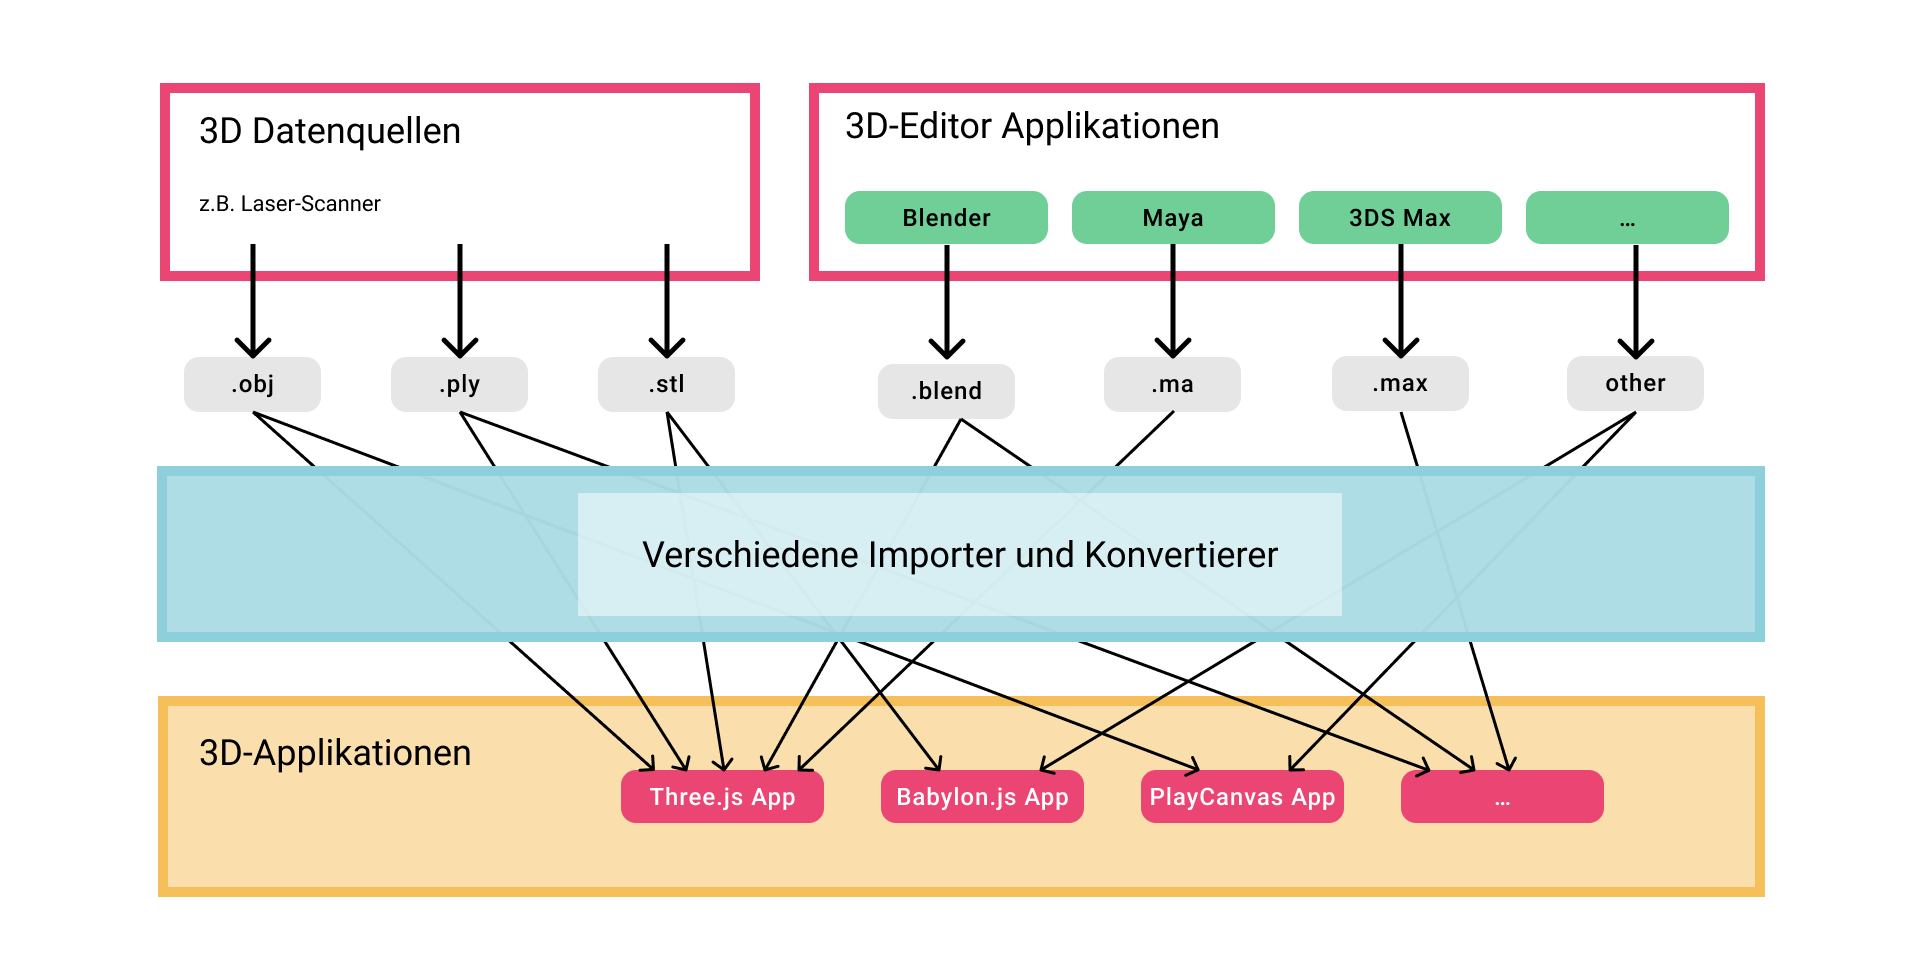
\includegraphics[width=0.8\columnwidth]{grundlagen/gltf/contentPipeline.png}
  \caption{Convertierungspipeline vor glTF \cite{gltf1Spec}}
  \label{fig:contentPipelineWithoutGltf}
\end{figure}

Durch die immer breiter werdende Nachfrage nach 3D-Applikationen wurde ein Format benötigt, dass zum einen Applikationsunabhängig verwendet und zum anderen performant im Web eingesetzt werden kann. \cite{gltf1Spec}
Durch diese Abstraktion können hunderte \e{converter} vermieden werden und nur wenige, sehr spezifische Dateiformate benötigen noch einen einzigen \e{converter}. Diese neue Pipeline ist in Abbildung \ref{fig:contentPipelineWithGltf} dargestellt. \cite{gltf1Spec}
\begin{figure}[H]
  \centering
  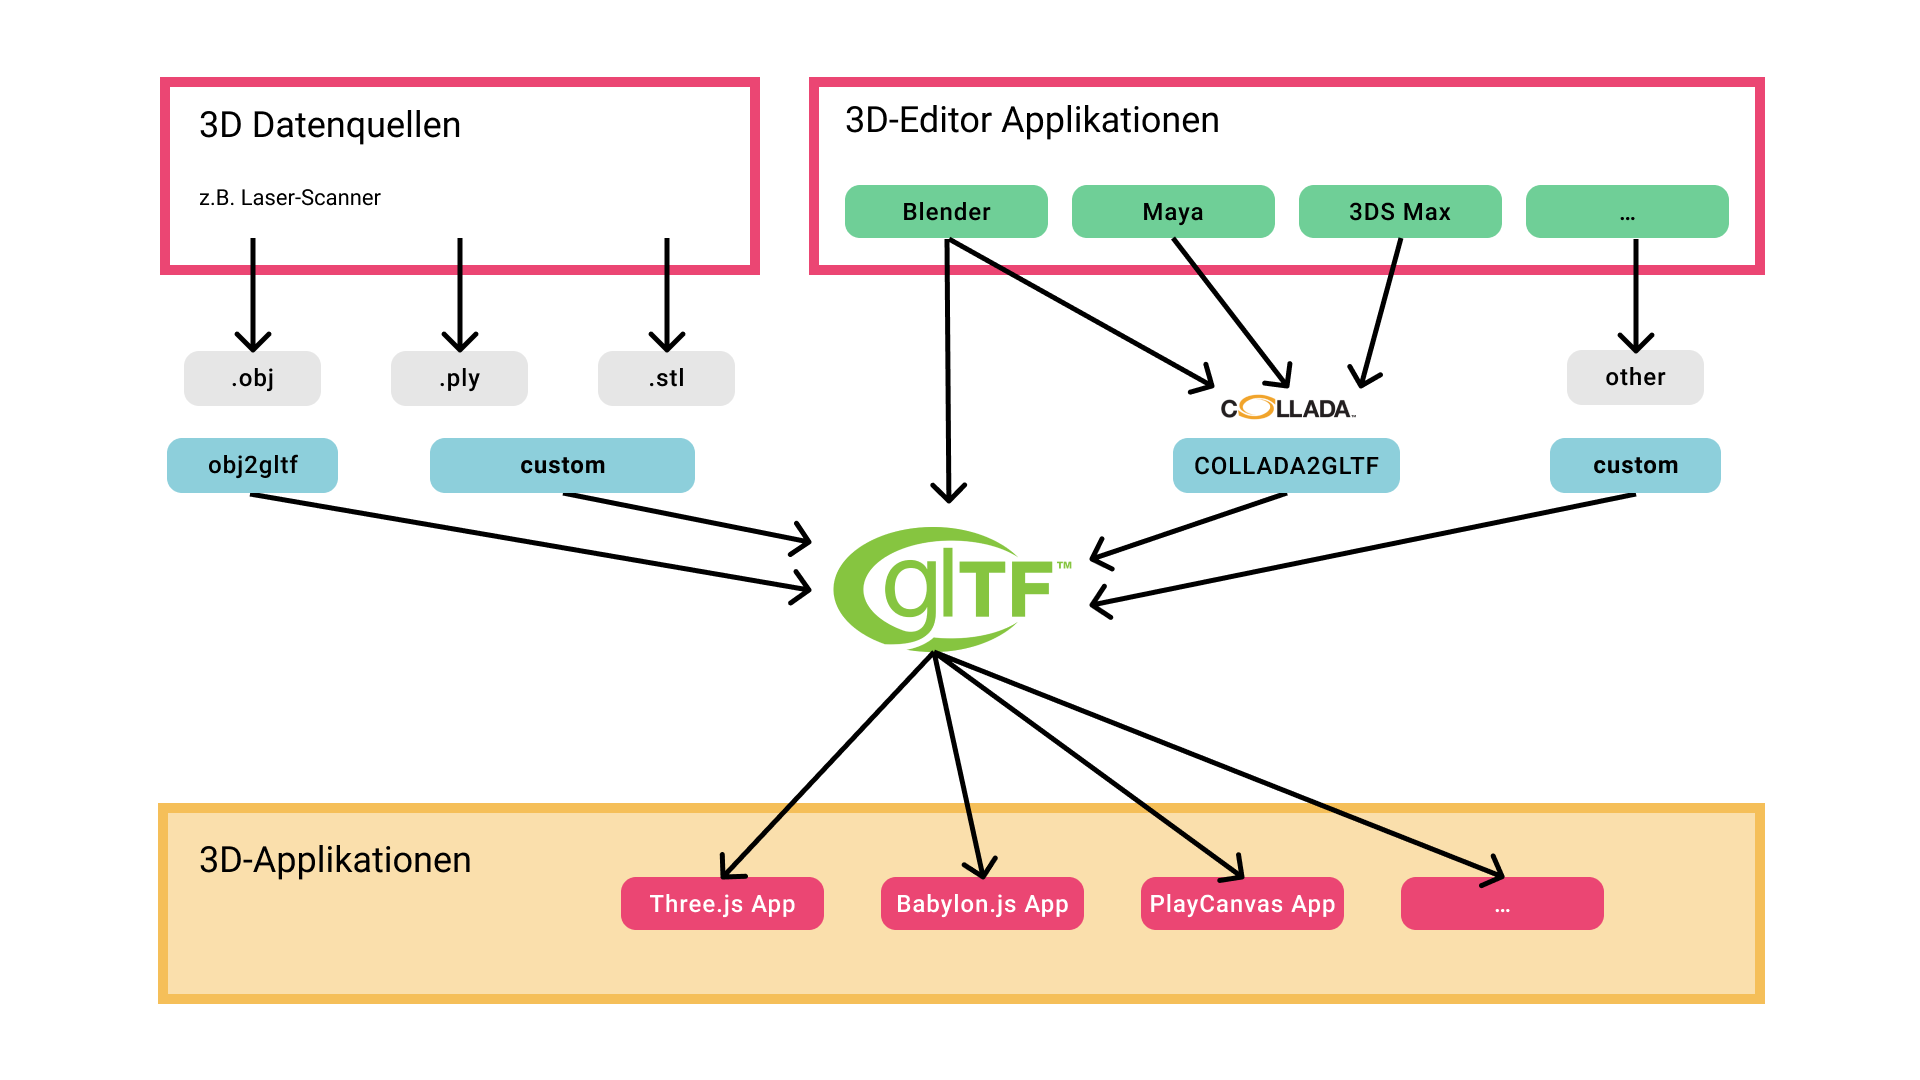
\includegraphics[width=0.8\columnwidth]{grundlagen/gltf/contentPipelineWithGltf.png}
  \caption{Convertierungspipeline mit glTF \cite{gltf1Spec}}
  \label{fig:contentPipelineWithGltf}
\end{figure}

Die Basisstruktur von glTF basiert auf JSON. Darin ist die komplette Szenerie des Modells beschrieben und in Abbildung \ref{fig:gltfDatastructure} aufgezeigt.\cite{gltf1Spec}
\begin{figure}[H]
  \centering
  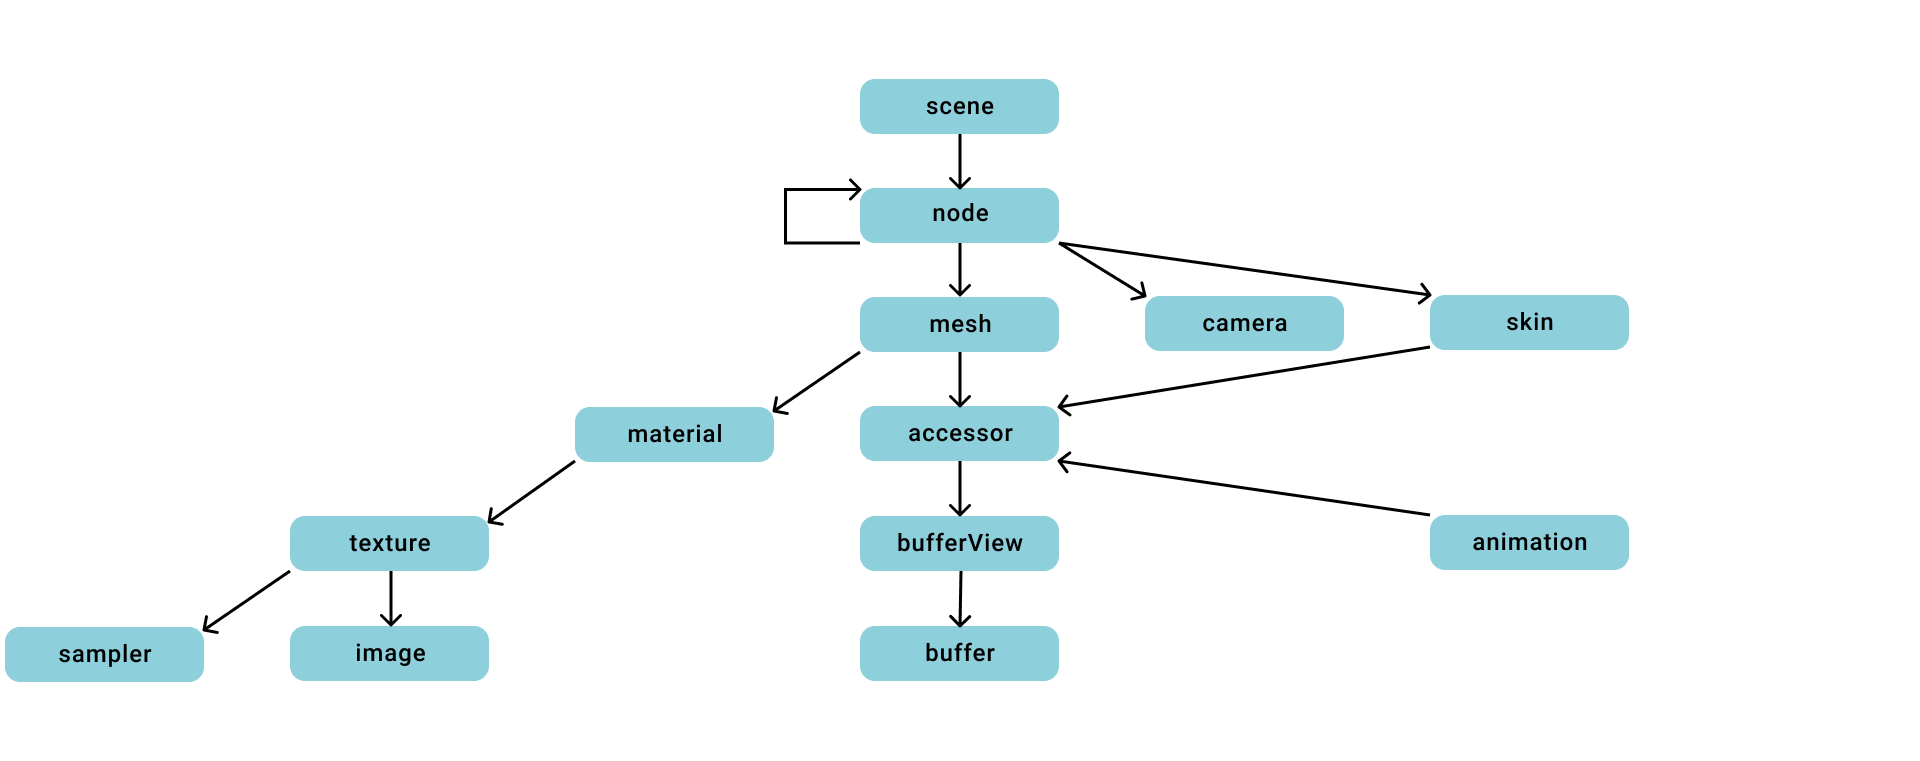
\includegraphics[width=0.8\columnwidth]{grundlagen/gltf/gltfJsonStructure.png}
  \caption{glTF Datenstruktur \cite{gltf1Spec}}
  \label{fig:gltfDatastructure}
\end{figure}

Die wichtigsten Elemente dieser Struktur kurz erläutert:
\begin{itemize}
  \item \textbf{Scene}: Einstiegspunkt der Szenerie und verweist auf alle Top-Level \e{nodes}.
  \item \textbf{Node}: Kann eine Transformation (Rotation, Translation oder Skalierung) beinhalten oder eine Kamera, \e{Skin}, Animation, ein \e{Mesh} oder \e{Childnodes} referenzieren.
  \item  \textbf{Mesh}: Beschreibt ein geometrisches Objekt und verweist auf \e{accessor}, welcher die effektiven geometrischen Daten beinhaltet und auf \e{material}, das beschreibt, wie das Objekt beim Rendern aussehen soll.
  \item \textbf{Accessor}: Verweis auf die Binärdaten (\e{BufferView}), welche die effektiven Eigenschaften für \e{meshes}, \e{skins} und \e{animations} kompakt beinhaltet.
  \item \textbf{BufferView}: Definiert eine Ansicht (Länge, Ort, Typ)auf einen \e{Buffer}.
  \item \textbf{Buffer}: Verweist auf einen Block von Binärdaten, welchen die effektiven Daten des 3D-Modells platzsparend beinhaltet.
  \item Weitere Elemente, welche im Rahmen dieser Arbeit nicht relevant sind und nicht im Detail betrachtet werden, sind: \e{camera}, \e{skin}, \e{material}, \e{animation}, \e{texture}.
\end{itemize}

\section{Transformation von Modellen}

Um ein Modell vereinfachen zu können, muss es verändert werden.
Diese Veränderungen können in Basis Operationen vereinfacht erläutert werden.

Im Folgenden werden Transformationen mithilfe einer 2D Visualisierung erläutert. Das Modell könnte jedoch ebenfalls im dreidimensionalen Raum sein – die Funktionsweise bleibt identisch.

Für die folgenden Beispiele wird jeweils das Modell aus Abbildung \ref{fig:transformationOriginal} verwendet.

\begin{figure}[H]
  \centering
  
\includegraphics[width=0.4\columnwidth]{grundlagen/transformationen/original.png}
  \caption{Modell Basis}
  \label{fig:transformationOriginal}
\end{figure}

\paragraph{Edge Collapse}
Hierbei werden zwei nebeneinanderliegende Vertices kombiniert, siehe Abbildung \ref{fig:transformationEdgeCollapse}.
Die Umkehrfunktion nennt man Vertex Split.

\begin{figure}[H]
  \centering
  \begin{subfigure}{.5\textwidth}
    \centering
    
\includegraphics[width=.8\linewidth]{grundlagen/transformationen/original.png}
    \caption{Modell Ausgangslage}
  \end{subfigure}%
  \begin{subfigure}{.5\textwidth}
    \centering
    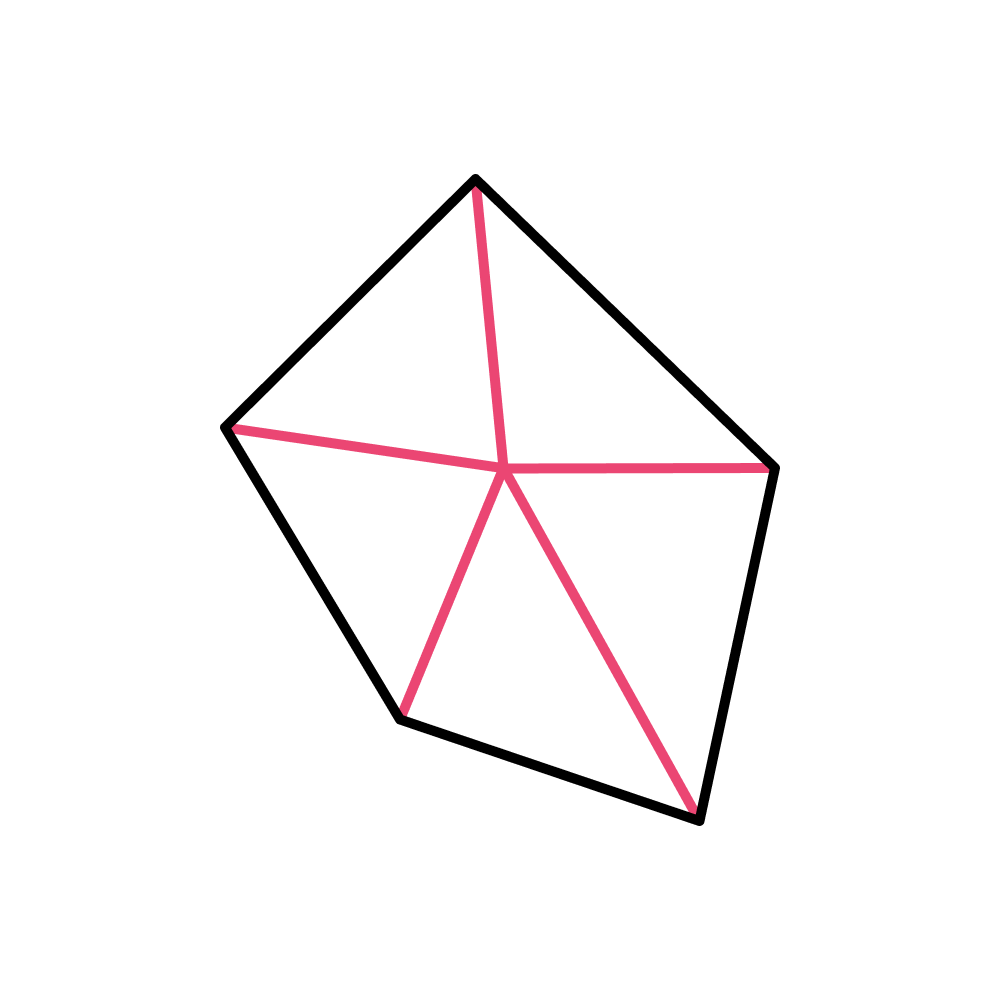
\includegraphics[width=.8\linewidth]{grundlagen/transformationen/edge-collapse.png}
    \caption{Edge Collapse}
  \end{subfigure}
  \caption{Transformation mittels Edge Collapse}
  \label{fig:transformationEdgeCollapse}
\end{figure}

\paragraph{Halfedge Collapse}
Hierbei wird ein Vertex direkt entfernt und alle Edges auf einen danebenliegenden Vertex zusammengelegt, siehe Abbildung \ref{fig:transformationHalfedgeCollapse}.

\begin{figure}[H]
  \centering
  \begin{subfigure}{.5\textwidth}
    \centering
    
\includegraphics[width=.8\linewidth]{grundlagen/transformationen/original.png}
    \caption{Modell Ausgangslage}
  \end{subfigure}%
  \begin{subfigure}{.5\textwidth}
    \centering
    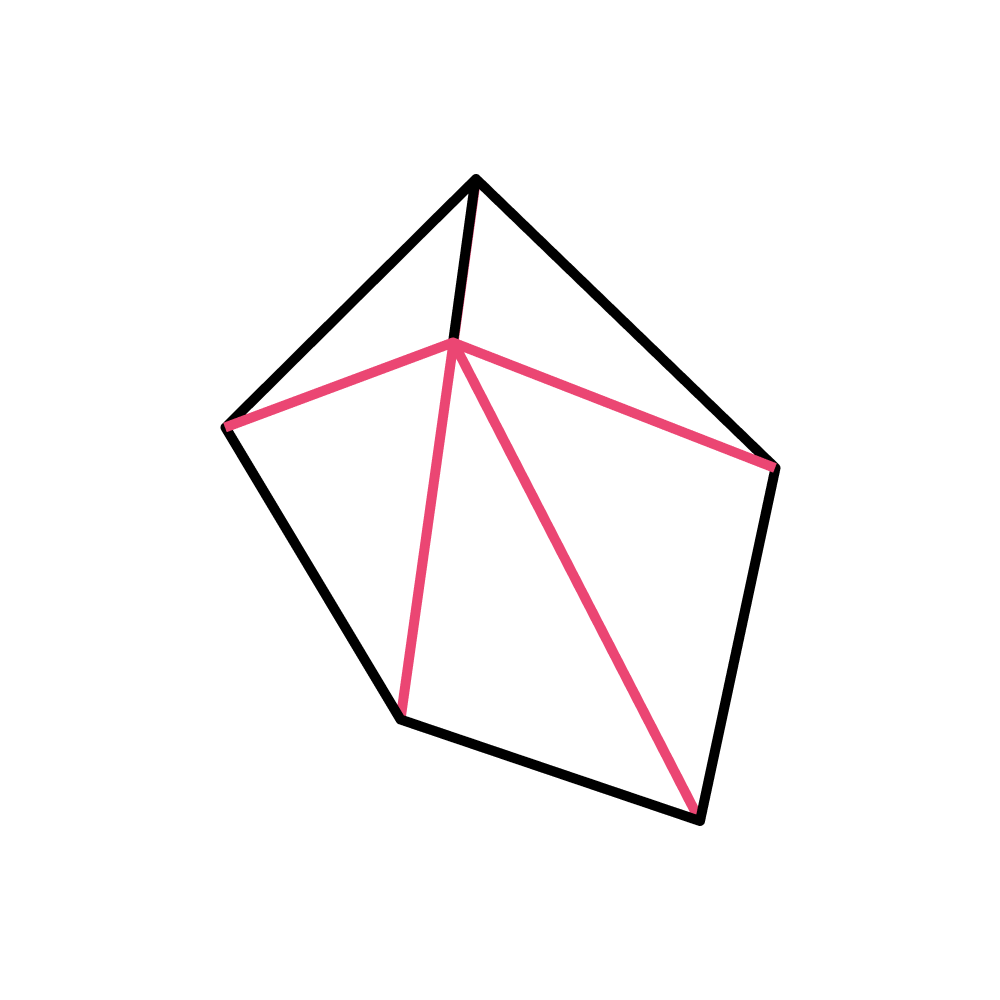
\includegraphics[width=.8\linewidth]{grundlagen/transformationen/half-edge-collapse.png}
    \caption{Halfedge Collapse}
  \end{subfigure}
  \caption{Transformation mittels Halfegde Collapse}
  \label{fig:transformationHalfedgeCollapse}
\end{figure}

\paragraph{Vertex Removal}
Hierbei wird ein Vertex entfernt und das Resultat neu \fgls{Trianguliert}{Verfahren, Polygone in Dreiecke aufzuteilen}.
In Abbildung \ref{fig:transformationVertexRemovalOriginal} wird der zentrale Vertex entfernt. Der neu triangulierte Polygon ist in Abbildung \ref{fig:transformationVertexRemovalFinal} ersichtlich.

\begin{figure}[H]
  \centering
  \begin{subfigure}{.5\textwidth}
    \centering
    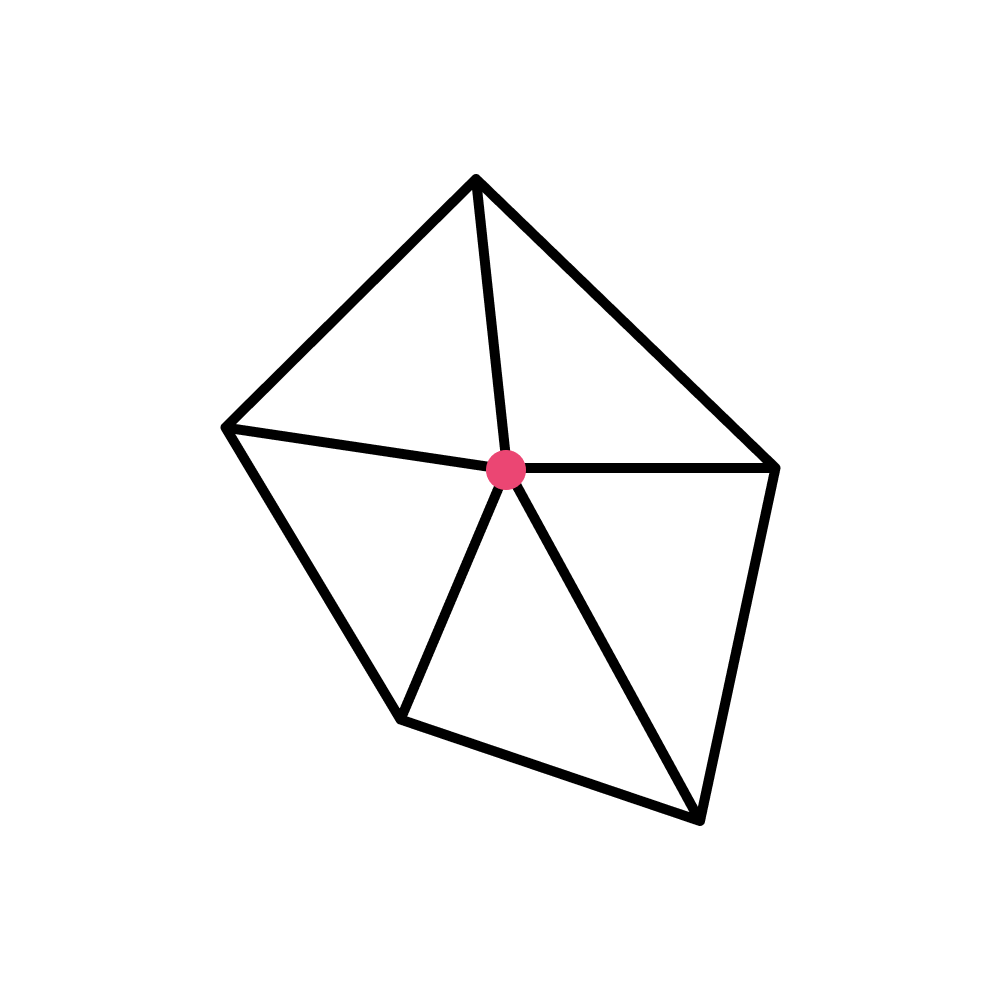
\includegraphics[width=.8\linewidth]{grundlagen/transformationen/vertex-removal-original.png}
    \caption{Modell Ausgangslage}
    \label{fig:transformationVertexRemovalOriginal}
  \end{subfigure}%
  \begin{subfigure}{.5\textwidth}
    \centering
    
\includegraphics[width=.8\linewidth]{grundlagen/transformationen/vertex-removal-final.png}
    \caption{Vertex Removal}
    \label{fig:transformationVertexRemovalFinal}
  \end{subfigure}
  \caption{Transformation mittels Vertex Removal}
  \label{fig:transformationVertexRemoval}
\end{figure}

\section{Graphics Pipeline}
Die Graphics Pipeline ist zuständig um eine definierte Szene auf einem Ausgabegerät zu visualisieren. Die verschiedenen Schritte werden im folgenden Abschnitt kurz erläutert. Es wird dabei ein simples 3D-Modell auf einen normalen 2D Display visualisiert. Die verschiedenen Schritte sind in Abbildung \ref{fig:renderingPipelineOverview} aufgezeigt.

\begin{figure}[H]
  \centering
  
\includegraphics[width=0.8\columnwidth]{grundlagen/pipeline/graphics-pipeline.png}
  \caption{Schritte einer Graphics Pipeline}
  \label{fig:renderingPipelineOverview}
\end{figure}

\paragraph{Applikation}
Im ersten Schritt wird die Szenerie aufbereitet, Modelle in den Arbeitsspeicher geladen, Positionen und Rotationen der Modelle definiert. Diese Schritte werden auf der CPU durchgeführt.

\paragraph{Geometrie}
Anschliessend werden die Definitionen an die Geometrie Pipeline geliefert. Diese ist zuständig um die Modelle auszurichten, die Beleuchtung zu bestimmen und die 2D Projektion vorzunehmen.

\paragraph{Rasterization}
Im letzten Schritt werden kontinuierliche Objekte zu diskreten Fragmenten verarbeitet. Der Anwender hat hierbei in vielen Engines die Möglichkeit, den Prozess mithilfe eines \fgls{Fragmentshaders}{Generiert Farbdefinition für ein einzelnes Pixel mit zugehörigem Tiefenwert} anzupassen.

\paragraph{Bildschirm}
Am Schluss wird das vom Rasterization Prozess generierte Bild auf dem Bildschirm dargestellt.

\section{Einführung LOD}
Als Level Of Detail (LOD) werden die verschiedenen Detailstufen bei der virtuellen Darstellung bezeichnet.
Dies wird verwendet, um die Geschwindigkeit von Anwendungen zu steigern, indem Objekte im Nahbereich detailiert angezeigt werden; wohingegen Elemente im Fernbereich deutlich vereinfacht dargestellt werden.

\subsection{Das Problem}
Geometrische Objekte können zu Komplex werden, um jederzeit performant und interaktiv gerendert zu werden.
Gerade wenn viele Objekte zur selben Zeit sichtbar sind, lohnt es sich, zu priorisieren und gewisse Objekte in reduzierter Qualität anzuzeigen.
Im Idealfall geschieht dies jedoch, ohne dass der Anwender dies bemerkt.

\subsection{Lösungsansätze}
In diesem Abschnitt werden mögliche Ansätze erklärt, welche helfen sollen, die Render-Perfomanz zu erhöhen. Diese Arbeit konzentriert sich jedoch auf den Ansatz von Level of Detail; die anderen Ansätze werden nur kurz erläutert.

\paragraph{Level of Detail}
Level of Detail auch bekannt als polygonale Simplifizierung, geometrische Simplifizierung oder Mesh Reduzierung basiert darauf, die Komplexität von Objekten zu reduzieren, welche weiter von der Kamera entfernt werden. Es gibt verschiedene Ansätze zur Generierung von LODs, welche in Abschnitt XY im Detail erläutert werden. Zudem braucht es einen berechenbare Methode, die Genauigkeit von Modellen zu definieren, um diese entsprechend anzuwenden. Schlussendlich ist dann noch zu definieren, ab wann welche Artefakte verwendet werden soll, basierend auf der Genauigkeit und der Komplexität.

\begin{figure}[H]
\centering
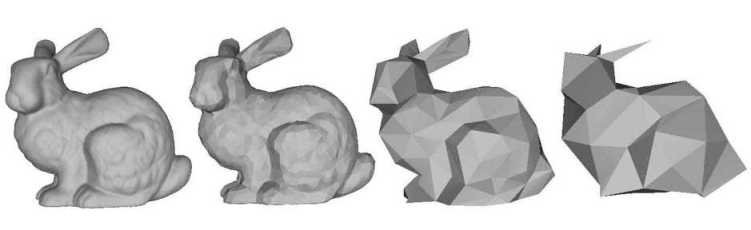
\includegraphics[width=0.8\columnwidth]{LODs-of-a-bunny-model-Courtesy-Stanford-3D-Scanning-Repository-From-left-to-right}
\caption{Level Of Detail Visualisierung vier Hasen}
\label{fig:LevelOfDetailVisualisierungvierHasen}
\end{figure}

Wie in der Abbildung \ref{fig:LevelOfDetailVisualisierungvierHasen} zu erkennen ist, wird von links nach rechts der Detailgrad und somit die Komplexität des Objektes reduziert. Sind es im Bild ganz links noch 69'451 Polygone, wird es bereits im ersten Schritt auf 2'502 Polygone reduziert. Dies ist eine enorme Reduktion von ca 96.5\%. Im dritten Schritt wird die Anzahl Polygone wiederum um ca. 90\% auf 251 reduziert. Schlussendlich hat das letzte Objekt noch 76 Polygone was knapp 0.1\% der ursprünglichen Anzahl entspricht.

\paragraph{Frustum culling}
Polygone, welche nicht im Kamera Frustum enthalten sind, werden bei dieser Methode nicht weiter prozessiert.
Dies reduziert die Anzahl Polygone drastisch.

\begin{figure}[H]
  \centering
  
\includegraphics[width=0.8\columnwidth]{grundlagen/Camera-Frustum.png}
  \caption{Camera Frustum}
  \label{fig:CameraFrustum}
\end{figure}

Ein Frustum ist eine geometrische Form, die einer Pyramide ähnelt, welcher die Spitze abgeschnitten wurde.
Das Kamera-Frustum bezeichnet den Raum, welcher von der Kamera aufgezeichnet wird. Dieser Breich startet eine gewisse Distanz von der Kamera entfernt und endet weit hinten wieder, da nicht bis ins unendliche Objekte sichtbar sind.
Wie in Abbildung \ref{fig:CameraFrustum} zusehen ist, beginnt das Kamera-Frustum in der nähe der Kamera und dehnt sich ein wenig aus bis es gegen Ende des Spektrums beschränkt wird.

\paragraph{Occlusion culling}
Polygone bzw. Objekte, welche komplett von anderen Objekten überdeckt werden, werden bei dieser Variante nicht prozessiert.

\paragraph{Backface culling}
\label{chap:backfaceCulling}
Bei dieser Methode wird berechnet welche Polygone zur Kamera orientiert sind.
Alle Polygone, welche in die andere Richtung zeigen werden nicht gezeichnet.
Dies ist nicht immer gewünscht, für die meisten Anwendungen ist diese Optimierung jedoch aktiviert.
Als Grundlage für die Berechnung werden die Normals der Vertices berücksichtigt.

\paragraph{Parallel rendering}
Auch bekannt unter Distributed Rendering ist der Einsatz von Techniken aus dem Parallel Programming in Visualisierungsanwendungen.

\paragraph{Image-based rendering}
In gewissen Fällen kann das Modellieren übersprungen werden. So kann anhand von Bildmaterial eine 3D-Illusion erzeugt werden.

\subsection{Verschiedene Ansätze zur Generierung von LOD Modellen}
Es gibt verschiedene Ansätze, 3D-Modelle mittels LOD zu vereinfachen. In diesem Abschnitt werden einige davon detaillierter erläutert so wie ihre Vor- und Nachteile aufgezeigt.

\paragraph{Diskrete LOD (DLOD)}
Bei diskreten LOD werden für ein detailliertes Modell mehrere weniger detaillierte Modelle verwendet.
Abhängig von der Distanz zum Betrachter wird das optimale Modell gewählt.
\begin{itemize}
  \pro Simplizität: Keine Anpassungen am \fgls{Scene Graph}{Objektorientierte Datenstruktur zur Beschreibung von 2D- oder 3D-Szenarien} notwendig
  \con Harte Grenzen: Veränderung des Objektes kann merkbar sein
  \con Kein Clustering möglich: Probleme bei sehr grossen oder vielen kleinen Modellen
\end{itemize}

\paragraph{Kontinuierliche LOD (CLOD)}
Im Gegensatz zu DLOD wird bei CLOD vereinfachende Veränderungen an einem Modell gespeichert.
\begin{itemize}
  \pro Weiche Grenzen: Interpolation zwischen Auflösungen ist möglich
  \con Runtime Performance
  \con Kein Clustering möglich
\end{itemize}

\paragraph{Hierarchische LOD (HLOD)}
Bei HLOD werden mehrere Objekte in einen Cluster gruppiert.
\begin{itemize}
  \pro Clustering möglich
\end{itemize}


\chapter{Vorgehen}
%%% Local Variables:
%%% mode: latex
%%% TeX-master: "../doc"
%%% coding: utf-8
%%% End:
% !TEX TS-program = pdflatexmk
% !TEX encoding = UTF-8 Unicode
% !TEX root = ../doc.tex
\section{Nutzen LOD}
Um den Nutzen von LOD quantifizieren zu können, wird in einer ersten Phase ein Benchmark aufgestellt.
Ziel ist es, das Laufzeitverhalten unter Einsatz eines optimierten Modells zu analysieren und somit den maximal möglichen Einfluss von LOD auf die Leistung klassifizieren zu können.

\subsection{Definition Benchmark}
Es gibt einige Ansätze, die das Durchführen eines Benchmarks vereinfachen. In diesem Abschnitt werden die verschiedenen erwägten Optionen erläutert und die Abgrenzungen aufgezeigt.

\paragraph{Browser Umgebung}
Um den Umfang des Benchmarks überschaubar zu halten, wurde ausschliesslich ein Benchmark für Google Chrome entwickelt.
Google Chrome basiert auf \fgls{Chromium}{Open Source Browser-Projekt. Grundlage von Browsern wie Google Chrome, Edge oder Opera}, dieselbe Engine, welche auch Microsoft Edge oder Opera verwenden.
Einen Benchmark basierend auf Google Chrome liefert somit auch Indizien für diese beiden Browser, auch wenn gewisse Abweichungen möglich sind.
Neben dem Marktführer Chrome sind Mozilla Firefox oder Safari von Apple ebenfalls Optionen. Jedoch wurde primär aufgrund des Marktanteils von total rund 70\% \cite{browserUsage} zugunsten von Google Chrome entschieden.

\paragraph{Automation}
Um die Tests durchzuführen, wird ein Testautomationstool benötigt; unter anderem der Einsatz von Selenium wurde in Erwägung gezogen.
Der Vorteil von Selenium ist insbesondere, dass der Benchmark für weitere Browser ausgeweitet werden könnte.
Da jedoch das Analysieren der GPU Daten stark vom System abhängig ist und dafür zusätzliche Komplexität notwendig wäre, wird in diesem Benchmark die im Google Chrome integrierten Chrome DevTools eingesetzt.
Selenium bietet zurzeit eine suboptimale Integration für das \emph{Chrome DevTools Protocol}.
\fgls{Puppeteer}{NodeJS Library, die eine API anbietet zum steuern von \gls{Chromium} oder Chrome über das Chrome DevTools Protocol}, eine weitere Option für die Automation, ist eine Bibliothek, die eine vereinfachte Schnittstelle zu einer Headless Chrome Instanz bietet.
Sie wird zudem direkt von Google entwickelt und bietet somit eine stabile Grundlage zur Kommunikation mit den DevTools.

\paragraph{Profiling}
Die Chrome DevTools erlauben es, ein detailliertes Profil einer Applikation anzulegen.
Im Profil befinden sich Informationen zu CPU/GPU Auslastung aber auch generelle Informationen bzgl. der \gls{Rendering Engine} werden gesammelt.
Die Analyse dieser Daten ermöglicht es, eine Aussage zum Laufzeitverhalten einer Applikation zu tätigen.

\paragraph{Testablauf}
Bei einem Testablauf werden folgende Schritte durchlaufen:

\begin{enumerate}
  \item Öffne Applikation in \emph{Headless Chrome} Instanz.
  \item Warte bis Seite geladen ist.
  \item Starte \emph{Profiling}.
  \item Warte $n$ Sekunden.
  \item Stoppe \emph{Profiling}.
  \item Werte Daten aus.
\end{enumerate}

Der Test erfasst kontinuierlich die \fgls{FPS}{Frames per Second. Bilder pro Sekunde. Gängige Art, die Performanz der \gls{Rendering Engine} zu messen}. Zudem wird aus dem \emph{Profiling} eine Kennzahl bzgl. der GPU Nutzung berechnet.

\paragraph{Analyse der Daten}
Um eine zuverlässige Aussage treffen zu können, wird der Vorgang mehrfach wiederholt. Für jeden Durchlauf wird der Median der \e{\gls{FPS}} Daten berechnet.
Anschliessend wird die Varianz der \e{\gls{FPS}} für die unoptimierten respektive optimierten Werte berechnet. Die Varianz dient als Kennzahl, um eine statistische Signifikanz nachweisen zu können. Abschliessend werden die Werte der beiden Versionen verglichen. Angestrebt werden sollten 60 \e{\gls{FPS}}. Wenn die unoptimierte Variante diesen Wert erreicht oder gar übersteigt, ist eine Optimierung nicht notwendig. Erreicht die optimierte Variante diesen Wert nicht, ist die Szenerie nach wie vor zu komplex. Ziel der Arbeit ist es, einen Algorithmus zu entwickeln, der für Szenerien unter 60 \e{\gls{FPS}} diese erhöht und im Idealfall auf ebendiesen Wert hebt.

\section{Vergleich LOD Systeme}
Die unterschiedlichen LOD Systeme bieten allesamt ihre Vor- und Nachteile. In diesem Schritt wird erläutert, welche Art LOD System in dieser Arbeit eingesetzt werden soll.

\section{Vergleich LOD Algorithmen}
Das diskrete LOD System ist für Grafiker und Entwickler die einfachste zu verwenden und deckt somit auch die breiteste Benutzerbasis und die meisten Anwendungsfälle ab. Aufgrund dessen, wird im Rahmen dieser Arbeit ein Algorithmus dieses Systems entwickelt und in den Entwicklungsprozess integriert.

\section{Pipeline Integration}
Die Lösung soll in eine wiederverwendbare und konfigurierbare Pipeline integriert werden.
In der Webentwicklung ist es üblich, über \fgls{CLI}{Command Line Interface – Kommandozeile} Arbeitsschritte zu automatisieren. Es soll demnach ein \e{\gls{CLI}} erstellt und auf \fgls{NPM}{Node Package Manager} öffentlich zugänglich gemacht werden, welches nahtlos in den Entwicklungsablauf integriert werden kann. Über eine Konfiguration soll angegeben werden können, wo nach den \e{.glTF} Dateien gesucht, wie die Output-Dateien benennt und in welchem Modus das Tool gestartet werden soll. Ebenso werden Algorithmus-Einstellungen in dieser Konfiguration gesetzt werden können. Es soll einfach zu bedienen, gut dokumentiert und gut gewählte Standardeinstellungen haben. Zudem soll das Tool im einmal Modus laufen können oder kontinuierlich sich ändernde Dateien neu optimieren.

\section{Automatische Generierung von Detail Levels}
Damit für den Endbenutzer die Konfiguration übersichtlich bleibt, soll der Einsatz von zum Beispiel heuristischen Methoden hilfreiche Basiskonfigurationen liefern.
Zum einen geht es hier um das Festlegen der Thresholds, aber auch das Definieren des Dezimierungs- / Vereinfachungsfaktors spielt eine wichtige Rolle.

\section{Levelwahl während Laufzeit}
Die optimale Levelwahl kann stark von der Laufzeitumgebung abhängig sein. So sollte zum Beispiel auf mobilen Geräten früher ein einfacheres Modell gezeigt werden als auf leistungsstarken Geräten.
Deshalb eignet sich eine Wahl der Levels zur Laufzeit, um ein optimales Erlebnis auf allen Geräten zu ermöglichen.
Nebst dem \e{\gls{CLI}} soll folglich auch ein Javascript-Modul bereitgestellt werden, welches das Laden von glTF Dateien übernimmt und basierend auf der erkannten Performanz das beste Level of Detail einspielen.

\chapter{Resultate}
%%% Local Variables:
%%% mode: latex
%%% TeX-master: "../doc"
%%% coding: utf-8
%%% End:
% !TEX TS-program = pdflatexmk
% !TEX encoding = UTF-8 Unicode
% !TEX root = ../doc.tex
\lipsum[1]

\chapter{Diskussion und Ausblick}
%%% Local Variables:
%%% mode: latex
%%% TeX-master: "../doc"
%%% coding: utf-8
%%% End:
% !TEX TS-program = pdflatexmk
% !TEX encoding = UTF-8 Unicode
% !TEX root = ../doc.tex
\lipsum[1]

\chapter{Verzeichnisse}
%%% Local Variables:
%%% mode: latex
%%% TeX-master: "../doc"
%%% coding: utf-8
%%% End:
% !TEX TS-program = pdflatexmk
% !TEX encoding = UTF-8 Unicode
% !TEX root = ../doc.tex
\printglossaries
\pagebreak
\begin{RaggedRight}
\bibliography{doc}
\bibliographystyle{deIEEEzhaw}
\end{RaggedRight}
\listoffigures
\listoftables


\appendix
\chapter{Anhang}
\label{ch:anhang}
%%% Local Variables:
%%% mode: latex
%%% TeX-master: "../doc"
%%% coding: utf-8
%%% End:
% !TEX TS-program = pdflatexmk
% !TEX encoding = UTF-8 Unicode
% !TEX root = ../doc.tex
\section{Aufgabenstellung}\label{sec:aufgabenstellung}
\begin{figure}[H]
\centering

\includegraphics[scale=0.6]{../ressources/Aufgabenstellung.pdf}
\end{figure}
\pagebreak
\section{Anhang 2}\label{sec:anhang_2}
\lipsum[1]
\end{document}